\documentclass[epsfig,10pt,fullpage]{article}

\newcommand{\LabNum}{4}
\newcommand{\CommonDocsPath}{../../common/docs}
\addtolength{\textwidth}{1.5in}
\addtolength{\oddsidemargin}{-0.75in}
\addtolength{\topmargin}{-0.75in}
\addtolength{\textheight}{1.5in}
\addtolength{\evensidemargin}{0.75in}
\setlength\parindent{0pt}
\raggedbottom

\usepackage{ae,aecompl}
\usepackage{epsfig,float,times}
\usepackage[hypcap]{caption}
\usepackage[pdftex, colorlinks]{hyperref}
\usepackage{graphicx}
\usepackage[usenames, dvipsnames]{color}
\usepackage{rotating}
\usepackage{tikz}
\usetikzlibrary{automata,positioning}
\usepackage{placeins}

\widowpenalty 10000
\clubpenalty 10000

\newcommand{\red}[1]{{\color{red}\sf{#1}}}
\newcommand{\green}[1]{{\color{green}\sf{#1}}}
\newcommand{\blue}[1]{{\color{blue}\sf{#1}}}
\definecolor{PineGreen}{rgb}{0.0, 0.47, 0.44}
\definecolor{ForestGreen}{rgb}{0.13, 0.55, 0.13}
\definecolor{Brown}{rgb}{0.59, 0.29, 0.0}

\newcommand{\UPDatePublished}{Oct 2021}
\newcommand{\versnum}{21.1} %version number quartus/AMP
\newcommand{\quartusname}{Quartus\textsuperscript{\textregistered} Prime}	
\newcommand{\UPTextBar}{For \quartusname{} \versnum{}}
\newcommand{\thisyear}{2021 } %for copyright
\newcommand{\company}{FPGAcademy.org}
\newcommand{\longteamname}{FPGAcademy.org}
\newcommand{\teamname}{FPGAcademy}
\newcommand{\website}{FPGAcademy.org}

\newcommand{\productAcronym}{AMP}
\newcommand{\productNameShort}{Monitor Program}

\newcommand{\productNameMedTM}{A Monitor Program}
\newcommand{\productNameMed}{A Monitor Program}

%\newcommand{\headerLogoFilePath}[1]{#1/FPGAcademy.png}

% listings is a package that supports encapsulating source code in LaTeX conveniently
\usepackage{listings}

\def\expandparam\lstinputlisting[#1]#2{\edef\tmp{\noexpand\lstinputlisting[#1]{#2}}\tmp}

%%%%%%%%%%%%%%%%%%%% Source Code Formatting %%%%%%%%%%%%%%%%%%%%
\definecolor{globalCommentColour}{rgb}{0.588,0.588,0.588}

%%%%%%%%%%%%%%%%%%%%%%%%%%%%%%%%%%%%%%%%%%%%%%%%%%%%
% Defining language style
% NiosII ASM
\lstdefinelanguage[NiosII]{Assembler} {
  morekeywords={add, addi, and, andhi, andi, beq, bge, bgeu, bgt, bgtu, ble,  bleu, blt, bltu, bne, br, break,
  bret, call, callr, cmpeq, cmpeqi, cmpge, cmpgei, cmpgeu, cmpgeui, cmpgt, cmpgti, cmpgtu, cmpgtui, cmple,
  cmplei, cmpleu, cmpleui, cmplt, cmplti, cmpltu, cmpltui, cmpne, cmpnei, custom, div, divu, eret, flushd,
  flushda, flushi, flushp, initd, initda, initi, jmp, jmpi, ldb, ldbio, ldbu, ldbuio, ldh, ldhio, ldhu, ldhuio,
  ldw, ldwio, mov, movhi, movi, movia, movui, mul, muli, mulxss, mulxsu, mulxuu, nextpc, nop, nor, or, orhi, ori,
  rdctl, rdprs, ret, rol, roli, ror, sll, slli, sra, srai, srl, srli, stb, stbio, sth, sthio, stw, stwio,
  sub, subi, sync, trap, wrctl, wrtcl, wrprs, xor, xori, xorhi, xori},
  morekeywords=[2]{.abort, .ABORT, .align, .app-file, .ascii, .asciz, .balign, .byte, .comm, .data, .def,
  .desc, .dim, .double, .eject, .else, .end, .endef, .endif, .equ, .equiv, .err, .extern, .file, .fill, .float,
  .global, .globl, .hword, .ident, .if, .include, .int, .irp, .irpc, .lcomm, .lflags, .line, .linkonce, .ln,
  .list, .long, .macro, .mri, .nolist, .octa, .org, .p2align, .psize, .quad, .rept, .sbttl, .scl, .section,
  .set, .short, .single, .size, .sleb128, .skip, .space, .stadb, .stabn, .stabs, .string, .symver, .tag,
  .text, .title, .type, .val, .uleb128, .word},
  morekeywords=[3]{et, bt, gp, sp, fp, ea, sstatus, ra, pc, status, estatus, bstatus, ienable, ipending, cpuid,
  exception, pteaddr, tlbacc, tlbmisc, eccinj, badaddr, config, mpubase, mpuacc},
  sensitive=t,
  alsoletter=.,
  morestring=[b]",
  morecomment=[s]{/*}{*/},
  morecomment=[l]\#,
}[keywords,comments,strings]
   
%% NOTE: morekeywords=[2] are GNU directives.
   
\definecolor{niosInstructionColour}{rgb}{0.000,0.608,0.000}
\definecolor{niosDirectiveColour}{rgb}{0.000,0.000,0.902}
\definecolor{niosSpecialRegColour}{rgb}{0.000,0.000,0.000}
\definecolor{niosStringColour}{rgb}{0.808,0.482,0.000}
   
%% NOTE: To make bold use: =\bfseries\color{<colour>}
\lstdefinestyle{defaultNiosStyle} {
  language=[NiosII]{Assembler},
  stringstyle=\color{niosStringColour},
  keywordstyle=\color{niosInstructionColour},
  keywordstyle=[2]\color{niosDirectiveColour},
  keywordstyle=[3]\itshape\color{niosSpecialRegColour}
}
%%%%%%%%%%%%%%%%%%%%%%%%%%%%%%%%%%%%%%%%%%%%%%%%%%%%

%%%%%%%%%%%%%%%%%%%%%%%%%%%%%%%%%%%%%%%%%%%%%%%%%%%%
% Defining language style
% ArmA9 ASM
\lstdefinelanguage[ArmA9]{Assembler} {
  morekeywords={ADC, ADD, ADDS, AND, ANDS, B, BAL, BEQ, BGE, BGT, BL, BLT, BIC, BKPT, BLX, BNE, BX, CDP, CLZ, CMN, CMP, EOR,
  EORS, LDC, LDM, LDR, LDRB, LDRBT, LDRH, LDRSB, LDRSH, LDRT, LSL, MCR, MLA, MOV, MOVW, MOVT, MRC, MRS, MSR, MUL, MVN, ORR, PLD,
  ROR, RSB, RSC, SBC, SMLAL, SMULL, STC, STM, STR, STRB, STRBT, STRH, STRT, SUB, SUBS, SWI, SWP, SWPB, TEQ, UMLAL,
  PUSH, POP, MOVS, RORS, LSR},
  morekeywords=[2]{.abort, .ABORT, .align, .app-file, .ascii, .asciz, .balign, .byte, .comm, .data, .def,
  .desc, .dim, .double, .eject, .else, .end, .endef, .endif, .equ, .equiv, .err, .extern, .file, .fill, .float,
  .global, .globl, .hword, .ident, .if, .include, .int, .irp, .irpc, .lcomm, .lflags, .line, .linkonce, .ln,
  .list, .long, .macro, .mri, .nolist, .octa, .org, .p2align, .psize, .quad, .rept, .sbttl, .scl, .section,
  .set, .short, .single, .size, .sleb128, .skip, .space, .stadb, .stabn, .stabs, .string, .symver, .tag,
  .text, .title, .type, .val, .vectors, .uleb128, .word},
  morekeywords=[3]{SP, PC, MIDR, CTR, TCMTR, TLBTR, MPIDR, ID_PFR0, ID_PFR1, ID_DFR0, ID_MMFR0, ID_MMFR1, ID_MMFR2,
  ID_MMFR3, ID_ISAR0, ID_ISAR1, ID_ISAR2, ID_ISAR3, ID_ISAR4, CCSIDR, CLIDR, AIDR, CSSELR, TTBR0, TTRB1, TTBR2, DACR,
  DFSR, IFSR, ADFSR, AIFSR, DFAAR, IFAR, ICIALLUIS, BPIALLIS, PAR, ICIALLU, ICIMVAU, BPIALL, DCIMVAC, DCISW, V2PCWPR,
  DCCVAC, DCCSW, DDIMVAC, DCISW, TLBALLIS, TLBIMVAIS, TLBIASIDIS, TLBIMVAAIS, TLBIALL, TLBIMVA, TLBIASID, TLBIMVAA,
  PMCR, PMCNTENSET, PMCNTENCLR, PMOVSR, PMSWINC, PMSELR, PMXEVTYPER, PMXEVCNTR, PMUSERENR, PMINTENSET, PMINTENCLR,
  PRRR, NRRR, PLEIDR, PLEASR, PLEFSR, PLEUAR, PLEPCR, VBAR, MVBAR, ISR, FCSEIDR, CONTEXTIDR, TPIDRURW, TPIDRURO, TPIDRPRW},
  sensitive=f,
  alsoletter=.,
  morestring=[b]",
  morecomment=[s]{/*}{*/},
  morecomment=[l]{//},
}[keywords,comments,strings]
   
%% NOTE: morekeywords=[2] are GNU directives.
   
\definecolor{armInstructionColour}{rgb}{0.000,0.608,0.000}
\definecolor{armDirectiveColour}{rgb}{0.000,0.000,0.902}
\definecolor{armSpecialRegColour}{rgb}{0.000,0.000,0.000}
\definecolor{armStringColour}{rgb}{0.808,0.482,0.000}
   
\lstdefinestyle{defaultArmStyle} {
  language=[ArmA9]{Assembler},
  stringstyle=\color{armStringColour},
  keywordstyle=\color{armInstructionColour},
  keywordstyle=[2]\color{armDirectiveColour},
  keywordstyle=[3]\itshape\color{armSpecialRegColour}
}
%%%%%%%%%%%%%%%%%%%%%%%%%%%%%%%%%%%%%%%%%%%%%%%%%%%%

%%%%%%%%%%%%%%%%%%%%%%%%%%%%%%%%%%%%%%%%%%%%%%%%%%%%
% Defining language style
% FPGAcademy ASM
\lstdefinelanguage{ASM}{
  morekeywords = [1]{mv, mvt, mvne, mvcc, add, sub, st, ld, and, b, bne, beq, bcc, bcs},
  morekeywords = [2]{word, define},
  keywordstyle = [1]\color{ForestGreen},
  keywordstyle = [2]\color{blue},
  sensitive = true,
  morecomment = [l]{//},
}

\lstset{
  language = ASM,
  basicstyle=\small\color{black}\ttfamily,
  commentstyle=\small\color{Brown}\itshape\ttfamily,
  showstringspaces=false,
  frame=none, %lines % boxed listings
  breaklines=true,
  breakatwhitespace=true,
  tabsize=3
}
%%%%%%%%%%%%%%%%%%%%%%%%%%%%%%%%%%%%%%%%%%%%%%%%%%%%

%%%%%%%%%%%%%%%%%%%%%%%%%%%%%%%%%%%%%%%%%%%%%%%%%%%%
% Defining language style
% Java
\definecolor{javaStringColour}{rgb}{0.808,0.482,0}
%%%%%%%%%%%%%%%%%%%%%%%%%%%%%%%%%%%%%%%%%%%%%%%%%%%%

%%%%%%%%%%%%%%%%%%%%%%%%%%%%%%%%%%%%%%%%%%%%%%%%%%%%
% Defining language style
% C
\definecolor{CStringColour}{rgb}{0.808,0.482,0}

\lstset{
  language = C,
  basicstyle=\small\color{black}\ttfamily, 
  commentstyle=\small\color{PineGreen}\itshape\ttfamily,
  keywordstyle=\small\color{blue}\bfseries\ttfamily,
  showstringspaces=false,
  frame=none, %lines % boxed listings
  breaklines=true,
  breakatwhitespace=true,
  tabsize=3
}
%%%%%%%%%%%%%%%%%%%%%%%%%%%%%%%%%%%%%%%%%%%%%%%%%%%%

%%%%%%%%%%%%%%%%%%%%%%%%%%%%%%%%%%%%%%%%%%%%%%%%%%%%
% Defining language style
% Verilog
\definecolor{verilogCommentColour}{rgb}{0.000,0.502,0.000}

\lstdefinestyle{defaultVerilogStyle} {
  language={Verilog},
  keywordstyle=\color{blue},
  commentstyle=\color{verilogCommentColour}
}
%%%%%%%%%%%%%%%%%%%%%%%%%%%%%%%%%%%%%%%%%%%%%%%%%%%%

%%%%%%%%%%%%%%%%%%%%%%%%%%%%%%%%%%%%%%%%%%%%%%%%%%%%
% Defining language style
% VHDL
\lstdefinestyle{defaultVHDLStyle} {
  language={VHDL},
  keywordstyle=\color{blue},
  commentstyle=\color{verilogCommentColour}
}
%%%%%%%%%%%%%%%%%%%%%%%%%%%%%%%%%%%%%%%%%%%%%%%%%%%%

%%%%%%%%%%%%%%%%%%%%%%%%%%%%%%%%%%%%%%%%%%%%%%%%%%%%
% Defining language style
% LaTeX
\lstdefinelanguage[LocalLaTeX]{TeX}[LaTeX]{TeX}{moretexcs={bf, it, sf, lstset},}

\lstdefinestyle{defaultLocalLatexStyle} {
  language=[LocalLatex]{TeX},
  keywordstyle=\color{blue}\bfseries,
  keywordstyle=[2]\color{blue},
  keywordstyle=[3]\color{blue}\bfseries
}
%%%%%%%%%%%%%%%%%%%%%%%%%%%%%%%%%%%%%%%%%%%%%%%%%%%%

%%%%%%%%%%%%%%%%%%%%%%%%%%%%%%%%%%%%%%%%%%%%%%%%%%%%
% Defining language style
% Default
\lstset{
  basicstyle=\small\color{black}\ttfamily,
  commentstyle=\small\color{globalCommentColour}\itshape\ttfamily,
  keywordstyle=\small\color{blue}\bfseries\ttfamily,
  showstringspaces=false,
  frame=none, %lines % boxed listings
  breaklines=true,
  breakatwhitespace=true,
  tabsize=3
}
%%%%%%%%%%%%%%%%%%%%%%%%%%%%%%%%%%%%%%%%%%%%%%%%%%%%


\hypersetup{
  pdftitle={Embedded Systems Lab Exercise \LabNum},
  linkcolor=blue,
  hyperindex=true,
  pdfauthor={FPGAcademy.org},
  pdfkeywords={FPGAcademy.org, FPGAcademy, Lab, Exercise, Embedded Systems},
  bookmarks,
  bookmarksopen=false,
  filecolor=blue,
  pdfstartview={FitH},
  urlcolor=blue,
  plainpages=false,
  pdfpagelabels=true,
  linkbordercolor={1 1 1} %no color for link border
}



\begin{document}

\centerline{\huge Embedded Systems}
~\\
\centerline{\huge Laboratory Exercise \LabNum}
~\\
\centerline{\large Using Character Device Drivers}
~\\

This exercise is a continuation of Laboratory Exercise 3, and is about character device
drivers. 

\section*{Part I}
\noindent
Write a character device driver that implements a {\it stopwatch}. The stopwatch 
should use the format MM:SS:DD, where {\it MM} are minutes, 
{\it SS} are seconds, and {\it DD} are hundredths of a second. The code for your driver 
should initialize the stopwatch time to 59:59:99, and should 
{\it decrement} the time each $1/100$ seconds. Your character device driver should 
provide the current stopwatch time via the file /{\it dev}/{\it stopwatch}. When the 
time reaches 00:00:00 the stopwatch should halt. 

~\\
\noindent
To keep track of time you should use a {\it hardware timer} module. The DE1-SoC Computer 
includes a number of hardware timers.  For this exercise use an interval timer implemented 
in the FPGA called {\it FPGA Timer0}. The register interface for this timer has the base 
address {\sf 0xFF202000}. As shown in Figure~\ref{fig:timer} this timer has six 16-bit 
registers. To use the timer you need to write a suitable value into the {\it Counter start value}
registers (there are two, one for the upper 16~bits, and one for the lower 16~bits of the 
32-bit counter value). To start the counter, you need to set the {\it START} bit in the 
{\it Control} register to~1. Once started the timer will count down to~0 from the initial 
value in the {\it Counter start value} register.  The counter will automatically reload this 
value and continue counting if the {\it CONT} bit in the {\it Control} register is~1. When the 
counter reaches~0, it will set the {\it TO} bit in the {\it Status} register to~1.
This bit can be cleared under program control by writing a~0 into it. If the 
{\it ITO} bit in the control register is set to~1, then the timer will generate an ARM* 
interrupt each time it sets the {\it TO} bit. The timer clock frequency is 100 MHz. 
The interrupt ID of the timer is 72. Follow the instructions in the tutorial {\it Using Linux 
on DE-series Boards} to register this interrupt ID with the Linux* kernel and ensure that it invokes 
your kernel module whenever the interrupt occurs.

~\\
\begin{figure}[htb]
	\begin{center}
	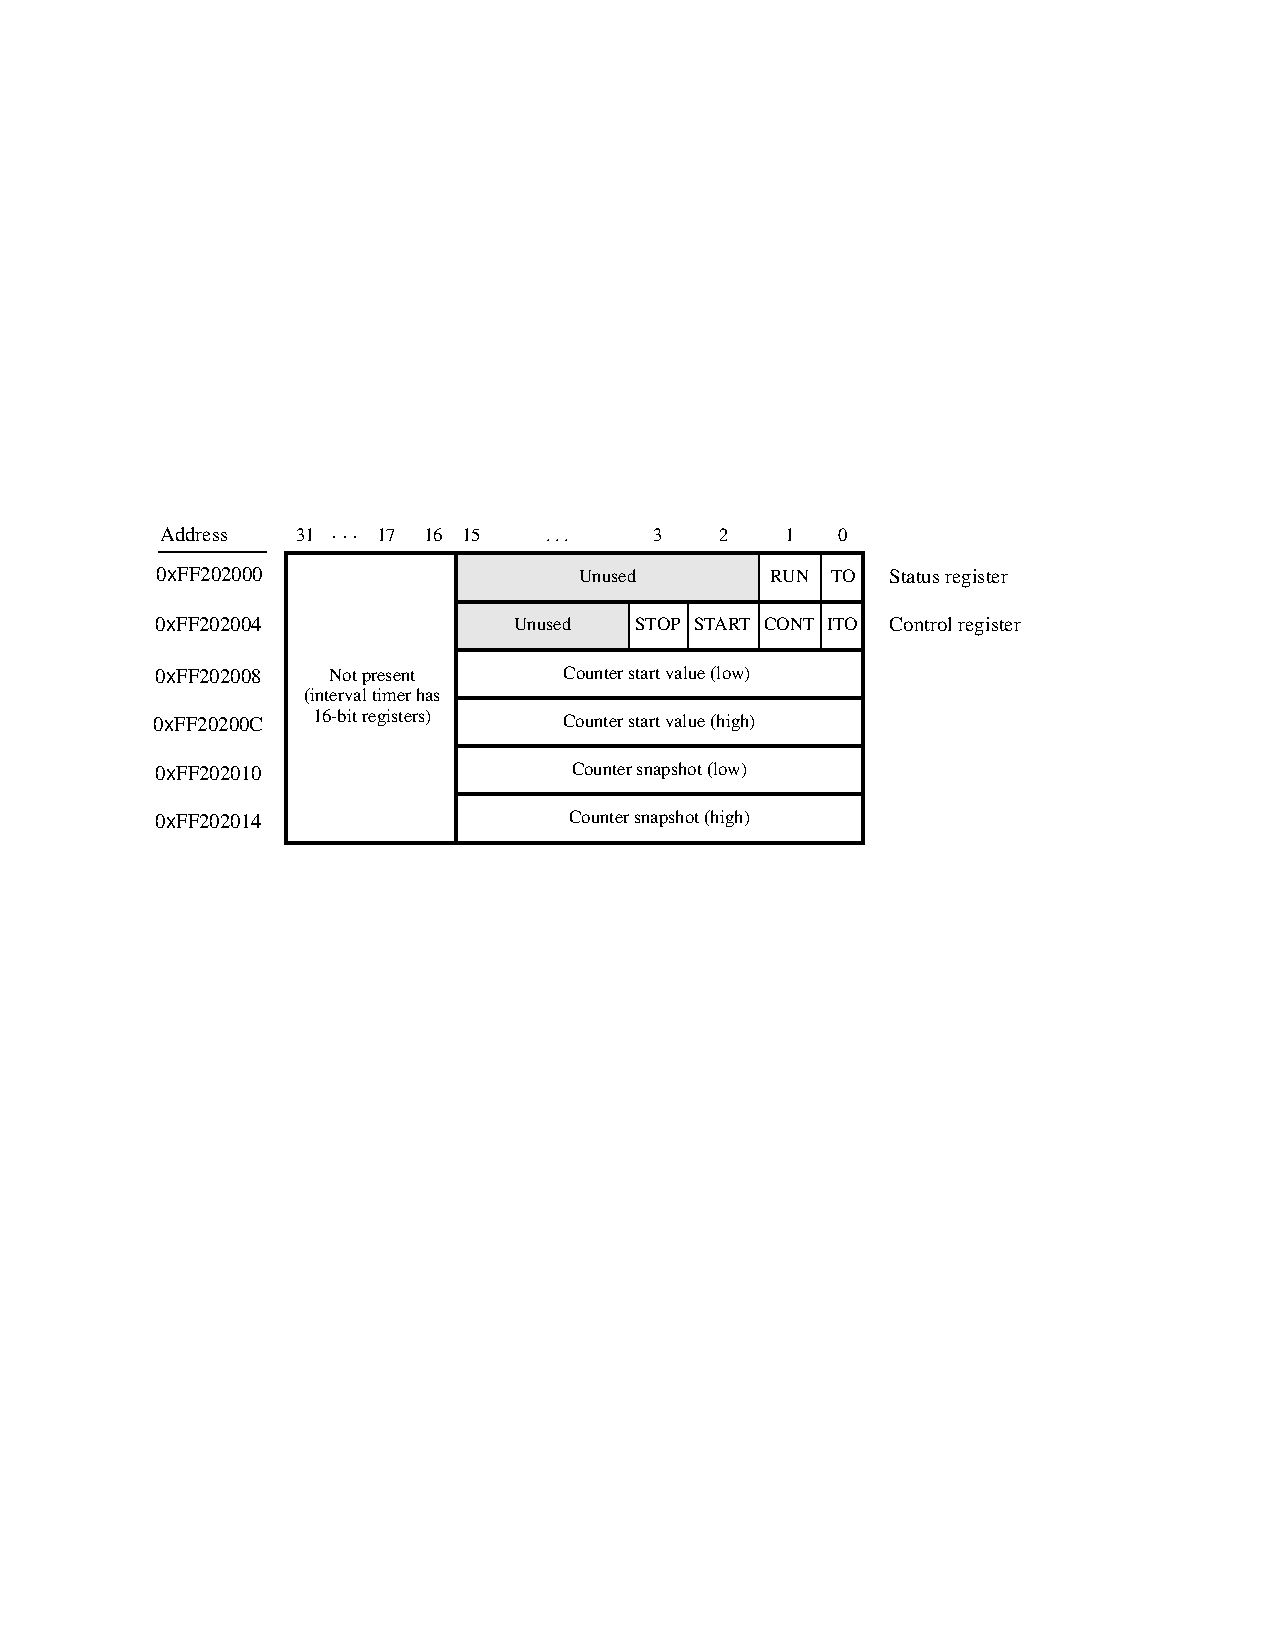
\includegraphics[scale=1]{figures/fig_interval_port.pdf}
	\end{center}
	\caption{The FPGA Timer0 register interface.}
\label{fig:timer}
\end{figure}

\noindent
Perform the following:

\begin{enumerate}
\item Create a file called {\it stopwatch.c} and type your C code into this file.

\item
Create a Makefile, compile your kernel module, and insert it into the kernel. 

\item
Test your character device driver by using the command \texttt{cat /dev/stopwatch}, which
should print the current stopwatch time.
\end{enumerate}

\section*{Part II}
\noindent
Augment your module from Part~I so that a user can control the stopwatch by writing
commands to the file /{\it dev}/{\it stopwatch}. Implement the following commands:
\texttt{stop}, \texttt{run}, and \texttt{MM:SS:DD}. The \texttt{stop} command causes the 
stopwatch to pause. The {\it run} command causes the stopwatch to operate normally, 
decrementing every $1/100$ seconds. The \texttt{MM:SS:DD} command is used to set the time.
For example, the command \texttt{echo 01:01:99 > /dev/stopwatch} sets the time to 1 
minute, 1 second, and 99 hundredths. 

~\\
\noindent
If you are using the DE1-SoC or DE10-Standard boards, which provide seven-segment displays,
then implement the two additional commands \texttt{disp}, and \texttt{nodisp}. Ignore these
commands if you are using the DE10-Nano board.
The \texttt{disp} command causes the stopwatch to show the time every $1/100$
seconds on the seven-segment displays HEX5-HEX0. The \texttt{nodisp} command turns off the
seven-segment display feature, and clears HEX5-HEX0. 

~\\
\noindent
Perform the following:

\begin{enumerate}
\item Create a new version of your {\it stopwatch.c} source-code file and write the code 
required for the new functionality. In addition to \texttt{open}, \texttt{release}, and 
\texttt{read} functions needed for Part I, you will need to add a \texttt{write} function. 
It should check which command has been written to the driver by the user, and take
appropriate action.

\item Use a Makefile to compile your kernel module. Ensure that the \texttt{stopwatch}
module from Part I is removed from the kernel, and then insert the new {\it stopwatch.ko} file. 

\item Test various commands to ensure that the character device driver works properly. 
\end{enumerate}

\section*{Part III}
\noindent
In this part we assume that the Linux system does not allow user-level code to access the
memory addresses of I/O devices. Instead, user-level code has to make use of device
drivers. Perform the following. 

\begin{enumerate}
\item Write a user-level program that controls the \texttt{stopwatch} driver from Part II. Your
program should execute in an endless loop, and should control the \texttt{stopwatch} using
the pushbutton KEY and switch SW ports, as follows. 
Pressing KEY$_0$ should toggle the \texttt{stopwatch} 
between the {\it run} and {\it pause} states. Other KEYs are used to set the \texttt{stopwatch}
time, based on the values of the switches SW. If you are using the DE1-SoC or DE10-Standard
board, set the \texttt{stopwatch} time as indicated in Table~\ref{tab:action1}. For the 
DE10-Nano board, which has fewer KEYs and SW switches, implement the actions given in 
Table~\ref{tab:action2}. To communicate with the KEY and SW ports, read from their
corresponding character device drivers. You may also want to display SW values on the LED
switches, using the character device driver for the LED port. For the character device drivers,
you could use either the drivers created as part of the solutions to Laboratory Exercise 3, 
or the drivers described in the tutorial {\it Using Linux on DE-series Boards}.
\item Compile your program using a command such as \texttt{gcc -Wall -o part3 part3.c}.
\item Ensure that the required character device drivers are inserted into the Linux kernel.
Test your program by controlling the \texttt{stopwatch} using the SW switches and pushbutton KEYs.
\end{enumerate}
\newpage
\begin{table}[h]
\caption{Setting the \texttt{stopwatch} for the DE1-SoC and DE10-Standard boards.}
~\\
\centering
\label{tab:action1}
\begin{tabular}{c|p{13cm}}
{\bf KEY} & {\bf Action} \\ \hline
\rule{0cm}{.375cm}{\it KEY}$_1$ & When pressed, use the values of the SW switches to set the \red{DD} part of the stopwatch time. The maximum value is \red{99} \\
{\it KEY}$_2$ & When pressed, use the values of the SW switches to set the \red{SS} part of the stopwatch time. The maximum value is \red{59} \\
{\it KEY}$_3$ & When pressed, use the values of the SW switches to set the \red{MM} part of the stopwatch time. The maximum value is \red{59} \\
\end{tabular}
\end{table}
\begin{table}[h]
\caption{Setting the \texttt{stopwatch} for the DE10-Nano board.}
\centering
\label{tab:action2}
\begin{tabular}{c|p{13cm}}
{\bf KEY} & {\bf Action} \\ \hline
\rule{0cm}{.375cm}{\it KEY}$_1$ &  If the stopwatch is running, just print the current time on
the Terminal window. But if the stopwatch is stopped, then set the time using the SW switch 
values. Set one stopwatch digit each time {\it KEY}$_1$ is pressed, in a specific sequence. 
For the first press, set the right digit of \red{DD}, for the second press set the left digit 
of \red{DD}, for the third press set the right digit of \red{SS}, and so on. After each 
press of {\it KEY}$_1$ print the current stopwatch time.
\end{tabular}
\end{table}

\section*{Part IV}
\noindent
For this part you are to write a user-level program that implements a {\it game}. Your program 
should use character devices drivers to communicate with the \texttt{SW} switches, 
\texttt{KEY} pushbuttons, \texttt{LED} lights, and \texttt{stopwatch}. The game
involves a series of mathematical problems, such as summations, presented to a user, with
a certain amount of time given to receive a correct answer. The game should perform as follows. 
In the first phase a default \texttt{stopwatch} time is shown on the seven-segment displays, 
and the user can change the displayed time by using the SW switches and KEYs. Use the
same scheme as for Part III to set the stopwatch.  Pressing KEY$_0$ starts the game. At this 
point the program should present a series of math questions that the user needs to answer 
within the \texttt{stopwatch} time. Answers should be entered through the command line. 
Incorrect answers to a question should be rejected, but the user should be allowed to 
try again as long as the time has not expired. 
After receiving a correct answer, the \texttt{stopwatch} should be reset and a new question asked. 
To make the game more interesting, you could increase the difficult 
of questions over time. At the end, when the user fails to respond within the \texttt{stopwatch}
time, some statistics about the results should be shown to the user (for example, you
could report the number of questions correctly answered, and the average time taken per question).

~\\
\noindent Perform the following.

\begin{enumerate}
\item Write the code that asks a series of math questions. An example of output that might
be produced by your game, with user responses, is shown below.

\begin{lstlisting}
Set stopwatch if desired. Press KEY0 to start
1 + 7 = 8
0 + 7 = 7
5 + 7 = 12
1 + 3 = 4
6 + 1 = 7
41 + 4 = 45
5 + 7 = 12
95 + 4 = 99
98 + 8 = 106
60 + 33 = 93
26 + 17 = 43
44 + 76 = 120
91 + 10 = 101
545 + 18 = 553
Try again: 563
972 + 3 = 975
572 + 75 = 627
Try again: 657
Time expired! You answered 17 questions, in an average of 2.73 seconds.
\end{lstlisting}

\item Compile your program using a command such as \texttt{gcc -Wall -o part4 part4.c}.
\item Run your program and make sure that the game functions properly.
\end{enumerate}

\vskip 0.5in
\noindent
\newpage
%%%%%%%%%%%%%%%%%%%%%%%%%%%%%%%%%%%%%%%%
%%% FPGAcademy Copyright Information %%%
%%%%%%%%%%%%%%%%%%%%%%%%%%%%%%%%%%%%%%%%

%Always put the copyright on a new page (clear page), with some vertical space from top
\clearpage
\vspace{1in}

\noindent

Copyright {\copyright} FPGAcademy.org. All rights reserved. FPGAcademy and the 
FPGAcademy logo are trademarks of FPGAcademy.org.  This document is provided 
"as is", without warranty of any kind, express or implied, including but not 
limited to the warranties of merchantability, fitness for a particular purpose 
and noninfringement. In no event shall the authors or copyright holders be 
liable for any claim, damages or other liability, whether in an action of 
contract, tort or otherwise, arising from, out of or in connection with the 
document or the use or other dealings in the document.
~\\
~\\
**Other names and brands may be claimed as the property of others.



\end{document}
